\chapter{Caso de Uso} \label{ch:cdu}

O presente capítulo visa explicar o caso de uso utilizado para validar o
sistema desenvolvido. Os casos de uso são simulações de parte da vida dos
personagens. No primeiro, eles encontram-se observando um jogo de futebol e
cada um torce para um time. No segundo, uma casa é simulada com quatro atores
e suas rotinas. Entretanto, antes desses casos serem abordados na
seção~\ref{ch:cdu:svc} e na seção~\ref{ch:cdu:home}
será falado como a ontologia foi testada juntamente com a plataforma
\emph{Jason}. A seção~\ref{ch:cdu:tbc} explica as ferramentas desenvolvidas
para o teste da base de crenças e, consequentemente, a ontologia. Elas são duas
uma interativa e outra não interativa que serve como uma especie de teste
unitário dos artefatos explicados no capítulo~\ref{ch:aec}.

\section{Teste da Base de Crenças} \label{ch:cdu:tbc}

Os testes da base de crenças tem como finalidade checar se a utilização normal
esta acontecendo da maneira esperada. Assim, eles fazem testes de inserção,
recuperação, remoção e listagem. Os testes foram escritos na linguagem
\emph{AgentSpeak}.

\begin{figure}
	\begin{center}
		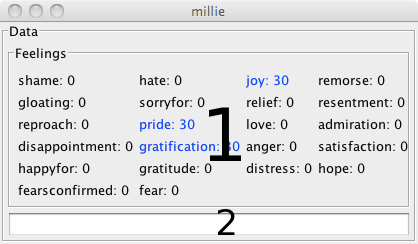
\includegraphics[width=70mm]{figuras/introductionDF.png}
	\end{center}
	\caption{Interface para mostrar os sentimentos dos agentes.}
	\label{fig:introducaoDF}
\end{figure}

A primeira aplicação de teste desenvolvida foi de maneira interativa conforme
pode ser observado na Figura~\ref{fig:introducaoDF}. A aplicação permite que o
usuário escreva as crenças do agente em um campo texto (área 2 na figura) e
esse é enviado diretamente para a base de crença do agente. A área 1 na mesma
figura é utilizada para demostrar a valência das emoções.
Essas informações podem aparecer em: preto, se não houve alteração com o ciclo
anterior; azul, se houve um aumento; vermelho, se houve uma diminuição do
valor.

\begin{figure}
	\begin{center}
		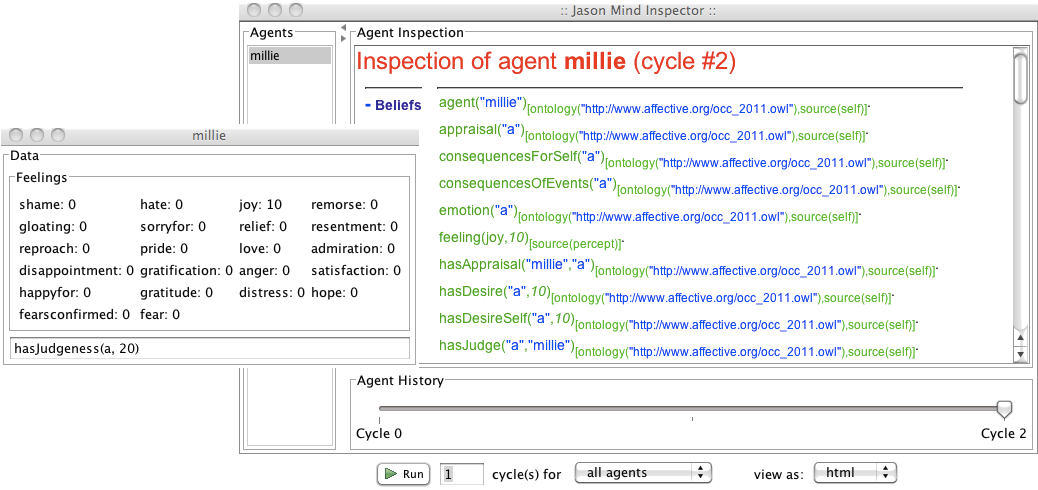
\includegraphics[width=150mm]{figuras/beforeLastInsertionOfPride.png}
		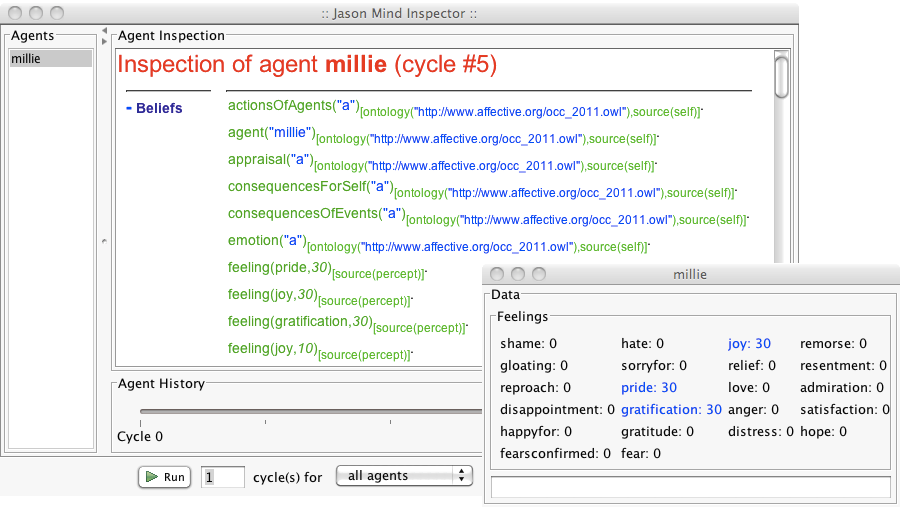
\includegraphics[width=150mm]{figuras/afterLastInsertionOfPride.png}
	\end{center}
	\caption{Exemplo de utilização criando uma emoção de orgulho.}
	\label{fig:testeJasonIntBase}
\end{figure}

Na Figura~\ref{fig:testeJasonIntBase} estão representados dois momentos da
criação de uma emoção de orgulho pelo usuário. Na parte de cima, o
agente tem configurado uma avaliação de e sobre si próprio. Além disso, a
avaliação tem probabilidade nula ou irrelevante e o desejo para si mesmo foi
considerado com o valor 10. Esse valor poderia ser qualquer número inteiro,
mas se fosse negativo ao invés de alegria (\emph{joy}) o resultado atual seria
sofrimento (\emph{distress}).

Na parte de baixo da Figura~\ref{fig:testeJasonIntBase} esta o resultado
obtido após a inserção da última crença para criação da emoção de orgulho.
Conforme pode ser visto,
foi necessário três ciclos deliberativos para o agente ter a percepção do
sentimento. Na verdade, essa percepção não veio de um novo ciclo de simulação
rodando e sim que o agente acredita que há um passo de simulação novo
então o processo emotivo foi disparado e as emoções criadas conforme
a configuração. Se fosse um passo normal da simulação, não se
teria na base de crenças duas percepções \emph{feeling} sobre uma emoção
porque a todo novo ciclo as percepções são apagadas. Cabe chamar atenção que
no sistema desenvolvimento não existe a ideia de decaimento dos valores com o
passar do tempo, para isso ser feito o agente deve reavaliar o problema e
atualizar os valores nas suas crenças.

Na Listagem~\ref{lst:testeJasonIntBase} pode ser observado uma configuração
para se rodar a presente aplicação\footnote{Veja a seção
\ref{sec-jason-overview} na página~\pageref{sec-jason-overview}
para ver uma introdução sobre esse tipo de arquivo.}. O ambiente na linha 3
espera que todos os agentes (quantidade informada no parâmetro 3) mandem
uma ação para prosseguir. O simulador espera pelo tempo (em milissegundos)
configurado no primeiro parâmetro por essas ações, caso não venha ignora o
agente e segue para o próximo ciclo. O segundo parâmetro permite informar
um número que representa o último passo de simulação e no quarto
parâmetro permite configurar se uma segunda ação enviada no mesmo passo de
simulação é para ser enfileirada ou resultar em erro (essa é a opção atual).

\begin{center}
    \begin{minipage}{130mm}
	\lstset{linewidth=130mm}
	\lstinputlisting[frame=trbl, caption=Arquivo de projeto do \jason para a
aplicação interativa de teste, label=lst:testeJasonIntBase]{../../sampletConsole/eoaus.mas2j}
    \end{minipage}
\end{center}

A agente millie configurada da linha 5 à 9 utiliza opções do \jason para
alterar a base de crença sendo utilizada (\emph{beliefBaseClass}),
arquitetura (\emph{agentArchClass}) e o raciocinador
(\emph{agentClass}). Essas alterações foram explicadas anteriormente
na seção~\ref{ch:p:ipjo}~(pág.~\pageref{ch:p:ipjo}).
Assim, para o presente exemplo a mudança da arquitetura na linha 7, única
classe não mencionada até agora, foi realizada para criar e atualizar a janela
que exibe os dados emotivos.

Cabe chamar a atenção que na linha 6 da Listagem~\ref{lst:testeJasonIntBase}
foi usada a ontologia afetiva desenvolvida somente. Assim, para o agente
utilizar as emoções ainda é necessário incluir as configurações de ativação
dos sentimentos via código. Uma amostra do código utilizado para se fazer isso
pode ser vista na Listagem~\ref{lst:testeJasonIntSetup} que mostra algumas
crenças iniciais do agente.

As crenças iniciais são carregados no agente no inicio da simulado. O processo
de carga segue conforme a regra da linha 6 da
Listagem~\ref{lst:testeJasonIntBase}. Sendo assim, a crença ``step'' como não
consta na ontologia será carregada na base de crenças padrão e as demais serão
criadas para popular a base de conhecimento. Esse processo fica transparente
para o código \emph{AgentSpeak}. Note que o usuário precisa definir o limite
para uma emoção virar sentimento em cada uma das 22 emoções.

\lstset{linewidth=80mm}
\begin{wrapfigure}{l}{80mm}
	\begin{lstlisting}[frame=trbl,
caption=Parte do código do agente para aplicação interativa de teste,
label=lst:testeJasonIntSetup]
step(0)[source(percept),source(self)].

agent(millie).

hasSetup(millie, setup1).
hasThreshold(setup1, 0).
hasThresholdType(setup1, "Joy").

hasSetup(millie, setup2).
hasThreshold(setup2, 0).
hasThresholdType(setup2, "Distress").
	\end{lstlisting}
\end{wrapfigure}

Nesse exemplo, os valores de limites estão sendo configurados com valoração
zero para que a potência e a valência sejam iguais. O agente somente conhece
a valência de uma emoção, ela é o valor da potência menos o limite de
ativação. Entretanto, tanto o limite de ativação quanto a potência não são
conhecidos pelo agente. Por exemplo, se o limite da pena (\emph{sorryFor}) é 6
e o valor atual é 8 então o sentimento com o valor 2 será criado sendo
expresso por uma crença da seguinte forma ``feeling("sorryFor",2).''.

%%%% fim da explicacao da aplicação interativa %%%%%

\begin{center}
    \begin{minipage}{140mm}
	\lstset{linewidth=140mm}
	\lstinputlisting[frame=trbl, caption=Arquivo de projeto do \jason para a
aplicação não interativa de teste,
label=lst:testeJasonNIBase]{../../sampletSummary/eoaus.mas2j}
    \end{minipage}
\end{center}

A aplicação não interativa utiliza a Listagem~\ref{lst:testeJasonNIBase} para
configurar o seu projeto. O ambiente especificado na linha 4 possui os mesmos
parâmetros do anterior com o acréscimo de um novo que indica uma ontologia.
Essa ontologia serve para o ambiente conhecer as rotinas dos agentes, como
deve ser desenhado o mapa à ser exibido e as posições iniciais de cada
agente. O agente millie aqui é o utilizado para os testes e os limiares de
ativação de emoção estão configurados para valores diferentes. Existe uma
variedade de testes para as propriedades de objeto ou de dados e para as
instâncias de classes, além de testes das conclusões esperadas.

\section{Assistindo um jogo de futebol} \label{ch:cdu:svc}

O caso de uso utilizado para demostrar a ontologia representa dois personagens
que se encontram no mesmo lugar e encontram-se assistindo ao mesmo jogo de
futebol. O jogo tem ao todo 60 turnos que representam os 90 minutos de um jogo
regulamentar. Em cada turno é sorteado um número randômico com probabilidade
de 1.67 de probabilidade para os times marcarem gol, isto é, há 98.33\% de
chance à cada turno de nada acontecer e o placar permanecer inalterado.

Esse exemplo aparentemente simples, propicia um cenário bastante rico para as
emoções por causa que um personagem pode ter diferentes emoções acontecendo.
Essas emoções são muitas vezes do ramo de consequências de eventos por esta
estar ligada com a desejabilidade do evento ou do ramo de ações de agentes que
tem haver com os padrões dos agentes. Assim, a mente dos atores que estão
assistindo ao jogo de futebol decidem no inicio da simulação os nomes de seus
times e ambos acreditam que venceram.

\begin{center}
    \begin{minipage}{140mm}
	\lstset{linewidth=140mm}
	\lstinputlisting[frame=trbl, caption=Arquivo de projeto do \jason para o
exemplo de futebol,
label=lst:soccer]{../../sampletSoccer/soccer.mas2j}
    \end{minipage}
\end{center}

A Listagem~\ref{lst:soccer} mostra o arquivo de projeto que cria dois agentes:
``watch1'' e ``watch2''. Cada um com seu próprio código fonte e,
dessa forma, cada um deles inclui em seus códigos as configurações
necessárias para utilizar o sistema. Um exemplo dessas configurações
é o limite de ativação para uma emoção virar sentimento. Outro exemplo é que
os times que participam do jogo são considerados pelos personagens como outros
agentes, assim o time que se torçe pode ser considerado ``amigo'' e o outro
``inimigo''.

Cabe salientar que cada um dos agentes realizam as mesmas avaliações sobre os
mesmos eventos. Esses eventos foram pensados como a marcação de um gol
(Listagem~\ref{lst:soccerGoal}), o estado atual do jogo
(Listagem~\ref{lst:soccerTeam}), o estado final do jogo
(Listagem~\ref{lst:soccerEnd1} e Listagem~\ref{lst:soccerEnd2}).
Esses são alguns exemplos escritos escritos na plataforma \jason para
fins de validação.

\begin{center}
    \begin{minipage}{120mm}
	\lstset{linewidth=120mm}
	\begin{lstlisting}[frame=trbl,
caption=Parte do código do agente referente à avaliação de gol,
label=lst:soccerGoal]
+?appraisalGoal
    :  goal(TEAM) & myPoints(TEAM, PF, _, _)
    <- ?fib(8-(PF+1), VAL);
       ?updateEmotion(prospectIrrelevant, "goal_myteam_pi", VAL);
       +removeEmotion("goal_myteam_pi").

+?appraisalGoal
    :  goal(TEAM) & myPoints(_, _, TEAM, PE)
    <- ?fib(PE+1, VAL);
       ?updateEmotion(prospectIrrelevant, "goal_enemyteam_pi", -VAL);
       +removeEmotion("goal_enemyteam_pi").

+?appraisalGoal
    : removeEmotion(INDIVIDIDUAL)
   <- ?removeEmotion(prospectIrrelevant, INDIVIDIDUAL);
      -removeEmotion(INDIVIDIDUAL).

+?appraisalGoal.
	\end{lstlisting}
    \end{minipage}
\end{center}

A Listagem~\ref{lst:soccerGoal} realiza o processamento das emoções sentidas
por um personagem quando um time marca um gol. Cada um dos planos criados
visam atender as 4 condições possíveis: gol do meu time, gol do adversário,
gol removido (não é mais percebido) e não houve gols. O plano da
linha 4 (\emph{updateEmotion}) e o da linha 15 (\emph{removeEmotion}, não
confundir o plano com a crença) serão explicados adiante por hora basta saber
que eles atualização ou removem as relações necessárias para a afetividade.

Na última listagem, as linhas 3 e 9 chamam um plano que consulta os números de
\emph{fibonacci}. Esse plano tem no primeiro parâmetro a posição do número na
sequência e o retorno correspondente. Entretanto, foi montado um plano que se
preocupa somente com a terceira à sétima posição e às demais posições são
assumidas com o valor 1. Os times quando jogam no simulador dificilmente
marcam mais que 5 gols então foi decidido limitar os números de
\emph{fibonacci} até a posição 7. Entretanto, valores de posição negativos ou
superiores à 7 terão retorno um. Cabe salientar que quando um gol é marcado
a favor do time que se torce o \emph{fibonacci} é usado de maneira
decrescente, isto é, o primeiro gol retornará a sétima posição, a segunda à
sexta e etc. No caso de gols do time adversário é utilizado o cálculo de
\emph{fibonacci} de maneira crescente. Logo, o valor 1 é retornado para os
dois primeiros gols, o terceiro terá valor 2 e assim por diante.

A Listagem~\ref{lst:soccerTeam} é similar à anterior. Ela é responsável por inserir uma
emoção de esperança no agente com valoração 50 e inicia o calculo de
realização do evento assumindo o valor positivo 1. Após, a cada gol percebido
do próprio time esse valor é incrementado em 10 e se o gol for do time
adversário é feito um decremento no mesmo valor. A emoção de esperança não
sofre alteração depois que é criada porque esta sendo considerado que as
emoções são baseadas na percepção dos eventos. Dessa forma, a esperança do
jogo ser ganho só termina quando há a percepção do encerramento do mesmo. Isso
vale para a emoção sentida em gols também.%, porém a emoção do gol só dura
%enquanto for percebido o gol.

\begin{center}
    \begin{minipage}{130mm}
	\lstset{linewidth=130mm}
	\begin{lstlisting}[frame=trbl,
caption=Parte do código do agente referente ao andamento do jogo,
label=lst:soccerTeam]
+?appraisalTeam
    :  not(hasLikelihood("team_hope_prn", PROB)) & step(STEP) & STEP < 10
    <- ?updateEmotion(prospectNotRealized, "team_hope_prn", 50);
       +realizedCalculation(1).

+?appraisalTeam
    :  goal(TEAM) & myPoints(_,_, TEAM, _) // ponto que nao eh meu
    &  realizedCalculation(CALC)
    <- -realizedCalculation(CALC);
       +realizedCalculation(CALC-10).

+?appraisalTeam
    :  goal(TEAM) & myPoints(TEAM, _, _,_) // ponto que eh meu
    &  realizedCalculation(CALC)
    <- -realizedCalculation(CALC);
       +realizedCalculation(CALC+10).

+?appraisalTeam.
	\end{lstlisting}
    \end{minipage}
\end{center}

\begin{center}
    \begin{minipage}{140mm}
	\lstset{linewidth=140mm}
	\begin{lstlisting}[frame=trbl,
caption=Parte do código do agente referente à avaliação do final do jogo para
as emoções de probabilidade,
label=lst:soccerEnd1]
+?appraisalEndMatch
    :  realizedCalculation(CALC) & match(_,_)
    &  hasLikelihood("team_hope_prn", PROB)
    &  feeling(hope, HOPEVAL)
    <- ?removeEmotion(prospectNotRealized, "team_hope_prn");
       ?updateEmotion(prospectRealized, "team_satisfaction_pr", HOPEVAL, CALC);
       -realizedCalculation(CALC).

+?appraisalEndMatch
    :  realizedCalculation(CALC) & match(_,_)
    &  hasLikelihood("team_hope_prn", PROB)
    <- ?removeEmotion(prospectNotRealized, "team_hope_prn");
       -realizedCalculation(CALC).

+?appraisalEndMatch.
	\end{lstlisting}
    \end{minipage}
\end{center}

Nas Listagens~\ref{lst:soccerEnd1}~e~\ref{lst:soccerEnd2} são realizadas
avaliações depois do termino do jogo. O jogo pode terminar empatado ou um dos
dois times ganhar. Entretanto, para a primeira listagem basta que o jogo tenha
terminado para uma atitude ser tomada. Essa atitude é a remoção da emoção de
esperança e a criação de uma nova emoção baseado em como foi o andamento do
jogo e no valor atual da esperança. Sendo assim, um personagem pode ficar
satisfeito ou desapontado.

Já, a Listagem~\ref{lst:soccerEnd2} permite um personagem sentir-se feliz
por ou com pena do resultado de seu time. Quando o time do personagem
tiver ganho o jogo ele pode sentir-se feliz ou neutro e quando o time perde
ele pode sentir-se com pena ou neutro da mesma forma. Esse valor de
neutralidade é porque o modelo de emoções só diz que a felicidade por alguém
ou a pena serão sentidas quando o merecimento e o desejo presumido sobre o
outro forem ambas positivas ou ambas negativas.

\begin{center}
    \begin{minipage}{140mm}
	\lstset{linewidth=140mm}
	\begin{lstlisting}[frame=trbl,
caption=Parte do código do agente referente à avaliação do final do jogo para
as emoções relacionadas com a consequência de eventos para outros,
label=lst:soccerEnd2]
+?appraisalEndMatchHappy
     : match(win, TEAM) & myPoints(TEAM, _, _, _)
     & not(hasAppraisal(NAME, "team_happy_foo"))
    <- .random(N); DE=math.round(N*20)-10; DT=20;
       ?updateEmotion(fortunesOfOthers, "team_happy_foo", DE, DT).

+?appraisalEndMatchHappy
     : match(lose, TEAM) & myPoints(TEAM, _, _, _)
     & not(hasAppraisal(NAME, "team_happy_foo"))
    <- .random(N); DE=math.round(N*20)-10;
       DT=-20; // eh negativo para implificar na emocao de pena
       ?updateEmotion(fortunesOfOthers, "team_happy_foo", DE, DT).

+?appraisalEndMatchHappy
     : match(draw, _) & myPoints(TEAM, _, _, _)
     & not(hasAppraisal(NAME, "team_happy_foo"))
    <- .random(N); DE=math.round(N*20)-10; DT=10;
       ?updateEmotion(fortunesOfOthers, "team_happy_foo", DE, DT).

+?appraisalEndMatchHappy.
	\end{lstlisting}
    \end{minipage}
\end{center}

As consultas de ``removeEmotion'', presentes nas listagens anteriores, recebem
o tipo de emoção e o nome do indivíduo que deve ser removido. Com base nessas
informações, as relações que foram outrora inseridas são removidas da base de
conhecimento e, consequentemente, da base de crenças. Um exemplo é amostrado
na Listagem~\ref{lst:removeSample} no qual são removidas às relações: de
merecimento, de desejo por outros, de qual pessoa esta sendo avaliada e de
quem esta avaliando.

\begin{center}
    \begin{minipage}{130mm}
	\lstset{linewidth=130mm}
	\begin{lstlisting}[frame=trbl,
caption=Amostra de remoção de emoção do tipo destino de outros,
label=lst:removeSample]
+?removeEmotion(fortunesOfOthers, INDIVIDUAL)
     : hasDeserved(INDIVIDUAL, OLDDE) & hasDesireOther(INDIVIDUAL, OLDDO)
     & hasPerson(INDIVIDUAL, TEAM)
    <- ?myName(NAME);
       -hasPerson(INDIVIDUAL, TEAM);
       -hasDeserved(INDIVIDUAL, OLDDE);
       -hasDesireOther(INDIVIDUAL, OLDDO);
       -hasAppraisal(NAME, INDIVIDUAL).

+?removeEmotion(fortunesOfOthers, INDIVIDUAL).
	\end{lstlisting}
    \end{minipage}
\end{center}

As consultas de ``updateEmotion'' funcionam de maneira parecida à
``removeEmotion''. Ela fazem a inserção das relações e caso já exista o
indivíduo removem e acrescentam novas relações para alterar o valor guardado.
Dessa forma, para a construção do exemplo tanto as atualizações como as
remoções foram agrupadas por grupo de emoções por causa que essa é a forma que
o próprio modelo \occ agrupa emoções com regras similares. A Listagem~\ref{lst:update}
mostra a regra para o tipo de emoções que tem haver com a consequência dos
destinos dos outros, isto é, as relações de merecimento, de nível de
desejo presumido e de quem esta avaliando e de qual pessoa esta sendo
avaliada.

\begin{center}
    \begin{minipage}{130mm}
	\lstset{linewidth=130mm}
	\begin{lstlisting}[frame=trbl,
caption=Amostra de código referente as atualizações de emoções do tipo destino de outros,
label=lst:update]
+?updateEmotion(fortunesOfOthers, INDIVIDUAL, DESERVED, DESIREOTHER)
     : team(TEAM) & not(hasPerson(INDIVIDUAL, TEAM))
    <- ?myName(NAME);
       +hasAppraisal(NAME, INDIVIDUAL);
       +hasPerson(INDIVIDUAL, TEAM);
       +hasDeserved(INDIVIDUAL, DESERVED);
       +hasDesireOther(INDIVIDUAL, DESIREOTHER).

+?updateEmotion(fortunesOfOthers, INDIVIDUAL, DESERVED, DESIREOTHER)
     : hasDeserved(INDIVIDUAL, OLDDE) & hasDesireOther(INDIVIDUAL, OLDDO)
    <- -hasDeserved(INDIVIDUAL, OLDDE);
       +hasDeserved(INDIVIDUAL, DESERVED);
       -hasDesireOther(INDIVIDUAL, OLDDO);
       +hasDesireOther(INDIVIDUAL, DESIREOTHER).

+?updateEmotion(fortunesOfOthers, INDIVIDUAL, DE, DO).
	\end{lstlisting}
    \end{minipage}
\end{center}

\section{Simulando uma casa} \label{ch:cdu:home}

O presente caso de uso tem por finalidade demonstrar as ontologias de rotinas
e preferências trabalhando junto da afetividade. Ele utiliza o ambiente e os
agentes de maneira diferente do caso anterior. O agente aqui não carrega os
limites de ativação dos sentimentos de crenças iniciais e sim da própria
ontologia. Todos seus valores estão configurados para a emoção virar
sentimento a partir do valor 20.

O ambiente utilizado nesse exemplo foi explicado brevemente quando introduzindo o
aplicativo de teste não-interativo. Esse ambiente carrega uma ontologia que
tem por finalidade conhecer as preferências e as rotinas dos agentes e por
construir uma visualização do ambiente no qual os atores desses agentes atuam.
Além disso, a cada passo de simulação as percepções são apagadas e as
preferências e rotinas do agente informadas.

Para a construção da visualização, cada um dos indivíduos do conceito
\emph{Place} são considerados como objetos que devem ser desenhados se
estiverem associados à uma dimensão. Assim, todos os objetos na tela são
desenhados a partir de retângulos. Além disso, esse conceito pode usar a
relação \emph{hasSetup} visando determinar que um objeto tem determinada
anotação ou, ainda, determinar que objetos fazem parte de um objeto maior. Por
exemplo, permitir que o agente saiba que o objeto sem visualização chamado
sala1 possui um armário, dois criados mundos, 2 duas camas e duas portas. Mas,
não conhece nenhuma das anotações desses objetos.
%Esse conhecimento serve para permitir que um agente que esta em um quarto se
%dirija para cozinha sem ter que conhecer previamente toda a casa.

\begin{figure}
	\begin{center}
		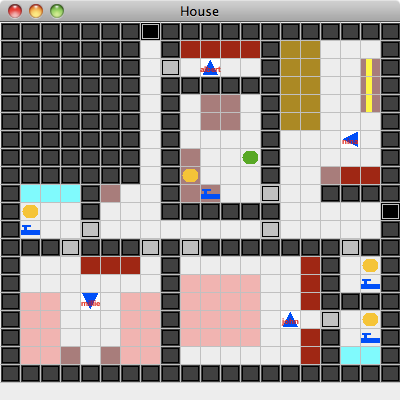
\includegraphics[width=10cm]{figuras/sims.png}
	\end{center}
	\caption{Interface de visualização da casa sendo simulada.}
	\label{fig:sims}
\end{figure}

A Figura~\ref{fig:sims} possui quatro atores diferentes chamados: millie,
albert, nina e john. Esses atores estão localizados em diferentes pontos da
casa e cada um pode ter sua própria orientação. No inicio da simulação eles
devem averiguar os objetos próximos para perceberem em qual sala se encontram
e depois decidem um objetivo próprio baseado em seu estado interno atual.
Muito provavelmente no inicio da simulação, os agentes tentaram ir para suas
respectivas camas dormirem para obter energia para o próximo dia.

O agente utiliza uma crença que o informar quanta energia ele possui. Quando
esse valor esta abaixo de um determinado limite a emoção de sofrimento começa
a ser utilizada e quanto mais baixa a energia maior o nível da emoção. A
emoção de alegria também pode ser disparada quando se esta com energia acima
do limite mencionado.

A atração e repulsa por um objeto pode ser usado...
